% Build: cd docs/reports/reconstruction/ms_ablation && latexmk -xelatex ms_ablation_mixed_20260422_zh.tex
\documentclass[a4paper, 11pt]{article}

\usepackage[margin=2.4cm]{geometry}
\usepackage{ctex}
\usepackage{amsmath,amssymb}
\usepackage{booktabs}
\usepackage{multirow}
\usepackage{array}
\usepackage{siunitx}
\usepackage{xcolor}
\usepackage{hyperref}
\usepackage{enumitem}
\usepackage{float}
\usepackage{graphicx}
\usepackage{caption}
\usepackage{subcaption}

\definecolor{goodgreen}{RGB}{34,139,34}
\definecolor{warnred}{RGB}{200,50,50}
\definecolor{fakegray}{RGB}{110,110,110}

\hypersetup{
  colorlinks=true,
  linkcolor=blue!60!black,
  citecolor=blue!60!black,
  urlcolor=blue!60!black,
}

\newcolumntype{R}[1]{>{\raggedleft\arraybackslash}p{#1}}

\title{\textbf{MS 消融实验 v2 · Beam-line 真空（Stage A$'$）\\
   ——三种几何情形下的 PDC 散度对比}}
\author{TBT \\ RIKEN 仁科中心 / DPOL 实验}
\date{2026 年 4 月 22 日}

\begin{document}
\maketitle

\begin{abstract}
\noindent
2026-04-21 的 Stage A 消融实验把 PDC2 命中 $\sigma_y$ 散度的 91--94\% 归给了“空气”，据此为 RK process-noise 修复（stage D）给出 $\sigma_{y,\mathrm{MS}}\approx 14$ mm 的输入。本次 Stage A$'$ 发现 stage A 所用“baseline”几何并不完全物理：Target $\to$ dipole 入射面（$\sim$0.68 m）以及 dipole yoke 内腔（$\sim$0.95 m）本应为束流真空，在原 Geant4 几何中却被世界空气填满。为此新增正交开关 \verb|/samurai/geometry/BeamLineVacuum|，把这 $\sim$1.63 m 上游段切为真空，再配合既有的 \verb|/samurai/geometry/FillAir|，构成三种几何情形：
\begin{itemize}[nosep,leftmargin=2em]
    \item \textbf{all\_air}：世界空气 + 上游段空气（原 stage A baseline）；
    \item \textbf{beamline\_vacuum}：世界空气 + 上游段真空（实验物理真实 baseline）；
    \item \textbf{all\_vacuum}：世界真空 + 上游段真空（参考，实验上不可达）。
\end{itemize}
在 $N=50$ ensemble、3 个 truth 动量点的 $627$~MeV/$c$ proton 注入下，三情形 $\sigma_y(\mathrm{PDC2})$ 分别为 $14.4$--$15.4$ mm、$6.8$--$8.2$ mm、$0.95$--$1.00$ mm，单调性完全成立。三段分解给出上游（虚假）和下游（真实）空气对 $\sigma_y(\mathrm{PDC2})$ 的贡献近 $1:1$（线性差 3 点平均分别为 $6.49$ 和 $6.51$ mm，quadrature 口径 $7.4$ mm）。由此 stage D 的 $\sigma_\mathrm{MS}$ 输入由 $14$ mm 修正到 $\sim$\textbf{7.4} mm（PDC2 y，quadrature）。本文档给出几何、数据、对比、与 Highland 核验，并附一节“已知数值伪影”：\texttt{all\_air} 与 stage A baseline 相差最高 +29\%（$\sigma_{\theta_y}$），源于新增 \texttt{vchamber\_cavity} LV 引起的 \texttt{G4eMultipleScattering} 步累积 topology 变化；\texttt{all\_vacuum} 与 stage A \texttt{no\_air} 则 bit-for-bit 相同，证明并非逻辑漏洞。
\end{abstract}

\tableofcontents
\newpage

% ============================================================
\section{背景与动机}
% ============================================================

DPOL 实验在 RIKEN SAMURAI 谱仪上进行，PDC 探测器负责测量 proton/deuteron 击中位置。RK 重建管线的 G4/Fisher 比较 \cite[§7.5]{rk_status}表明 PDC2 的 $\sigma_y\sim 11$--$15$ mm 不能由丝室本征分辨率（$\sim 0.2$ mm）解释，必须有多重库仑散射（multiple Coulomb scattering，MS）参与。Stage A 通过把 Geant4 世界材质 \texttt{FillAir} 从 \texttt{true} 切到 \texttt{false}（world 变真空），发现 $\sigma_y(\mathrm{PDC2})$ 塌到 $\sim 1$ mm，据此把剩余 $\Delta\sigma$ 归给“空气”。

但 Stage A 的“baseline”几何存在一处潜在错误：\textbf{束流管 / 磁铁真空腔的内部本该是真空，不是空气}。SAMURAI 偶极磁铁的束流腔（\texttt{vchamber}）是一个真空容器，其入射端通过法兰连接到靶真空仓，出射端通过 exit window 连到下游大气段。在 stage A 的代码路径里：

\begin{itemize}[nosep]
  \item \texttt{VacuumUpstream}（靶 $\to$ 偶极入射面）构造类存在于代码中但未被实例化；
  \item 偶极 yoke 内腔在几何里由 \texttt{G4SubtractionSolid} 从 yoke 中挖空，但挖空区域直接暴露于母体积（\texttt{expHall\_log}），材质继承世界材质（即当 \texttt{FillAir=true} 时为空气）。
\end{itemize}

\noindent 因此 stage A 的 \texttt{baseline} 中，粒子从靶出射到抵达下游 \texttt{exit window} 之前，多了 $\sim$1.63 m 的“不该存在的空气段”。Stage A 的 $94\%$ 故而混入了这段虚假空气贡献；stage D 的 $14$ mm $\sigma_\mathrm{MS}$ 输入相应偏大。

Stage A$'$ 的目的是：(i) 新加 \verb|BeamLineVacuum| 开关把上游 $\sim$1.63 m 真空化；(ii) 跑三情形比较；(iii) 把 PDC2 $\sigma_y$ 的“空气成分”严格拆成 \textbf{上游虚假} 与 \textbf{下游真实} 两部分；(iv) 修正 stage D 的噪声幅度输入。

% ============================================================
\section{几何修改}
% ============================================================

\subsection{新增的 Messenger 命令}

在 \texttt{DeutDetectorMessenger} 中新增：
\begin{center}
\begin{tabular}{ll}
\toprule
命令 & 语义 \\
\midrule
\verb|/samurai/geometry/FillAir <bool>|       & （已有）世界体积填料：空气/真空 \\
\verb|/samurai/geometry/BeamLineVacuum <bool>| & （新加）上游段+yoke 内腔：真空/继承 world \\
\bottomrule
\end{tabular}
\end{center}

默认值 \verb|BeamLineVacuum=false| 保证对未显式设置该项的现有 macro 行为保持\emph{名义}一致（参见 §\ref{sec:artifact} 关于数值伪影的讨论）。

\subsection{C++ 改动}

\begin{enumerate}[nosep]
  \item \textbf{DeutDetectorConstruction}：新增 \texttt{fBeamLineVacuum} 成员；若为 true，实例化并摆放 \texttt{VacuumUpstreamConstruction}（该类已存在，原未被 wire）；无论如何都调用 \texttt{fDipoleConstruction->SetBeamLineVacuum(.)}。
  \item \textbf{DipoleConstruction}：原 yoke 几何 = \texttt{G4Box} $-$ \texttt{vchamber\_cavity\_sol}（cavity 由 \texttt{G4UnionSolid} 构造为 box + trap）。改动：在从 yoke subtractive 构造的同时，\emph{显式地} 把该 cavity 作为一个独立 \texttt{G4LogicalVolume} 放入 yoke 内——
  \[
      \text{cavity 材质} = \begin{cases}
          \texttt{G4\_Galactic}, & \texttt{fBeamLineVacuum}=\text{true}\\
          \text{world material}, & \text{否则}
      \end{cases}
  \]
  \texttt{checkOverlaps=true}。
  \item \textbf{VacuumUpstreamConstruction}：只在 \texttt{fBeamLineVacuum=true} 时被放置；几何为从靶前端到 dipole 入射法兰的真空圆柱/圆台。
\end{enumerate}

\textbf{设计选择}：物理上 \texttt{BeamLineVacuum=false} 与旧代码\emph{名义}等价（yoke 内腔填料 = world material = 空气，与原先 subtractive 留白后继承世界材质等价）。我们后续会量化 Geant4 MSC 数值 topology 变化带来的 $\sim 10\%$ 量级数值漂移（§\ref{sec:artifact}）。

\subsection{宏文件}

\begin{center}
\begin{tabular}{lll}
\toprule
条件 & 宏文件 & 关键行 \\
\midrule
\texttt{all\_air}         & \verb|geometry_B115T_pdcOptimized_20260227_target3deg.mac|       & \texttt{FillAir true}（无 BeamLineVacuum） \\
\texttt{beamline\_vacuum} & \verb|geometry_B115T_pdcOptimized_20260227_target3deg_mixed.mac| & \texttt{FillAir true}, \texttt{BeamLineVacuum true} \\
\texttt{all\_vacuum}      & \verb|geometry_B115T_pdcOptimized_20260227_target3deg_noair.mac| & \texttt{FillAir false}（等价于 BeamLineVacuum 不设） \\
\bottomrule
\end{tabular}
\end{center}

三个宏位于 \verb|configs/simulation/DbeamTest/detailMag1to1.2T/|。前后相互间只差 1 行（差分经单元测试 \verb|scripts/analysis/ms_ablation/tests/test_macro_diff_mixed.sh| 校验）。

% ============================================================
\section{飞行路径几何}
\label{sec:path}
% ============================================================

粒子从靶出发到抵达 PDC2 的典型飞行路径按几何分段列于表~\ref{tab:flight_path}。这些长度取自 \verb|geometry_B115T_pdcOptimized_20260227_target3deg.mac| 的 GDML/构造参数，数值精度 $\pm 5\%$。

\begin{table}[H]
\centering
\caption{粒子飞行路径分段与三情形下的材质状态。前两段（$\sim$1.63 m）是 stage A$'$ 新 switch \texttt{BeamLineVacuum} 控制的上游段，后两段（$\sim$1.80 m）是已有 \texttt{FillAir} 控制的下游空气段。}
\label{tab:flight_path}
\begin{tabular}{lrccc}
\toprule
路段 & 长度 & \texttt{all\_air} & \texttt{beamline\_vacuum} & \texttt{all\_vacuum} \\
\midrule
Target $\to$ dipole 入射面        & $\sim 0.68$ m & \textcolor{warnred}{空气（虚假）}  & 真空 (VacuumUpstream) & 真空 \\
Dipole yoke 内腔（沿弧）          & $\sim 0.95$ m & \textcolor{warnred}{空气（虚假）}  & 真空 (vchamber\_cavity) & 真空 \\
\midrule
Dipole 出射 $\to$ ExitWindow      & $\sim 1.45$ m & 真空 (VacuumDownstream)  & 真空 & 真空 \\
ExitWindow $\to$ PDC1             & $\sim 0.80$ m & \textcolor{goodgreen}{空气（真实）} & \textcolor{goodgreen}{空气} & 真空 \\
PDC1 $\to$ PDC2                   & $\sim 1.00$ m & \textcolor{goodgreen}{空气（真实）} & \textcolor{goodgreen}{空气} & 真空 \\
\midrule
\textbf{上游空气合计} (\texttt{upstream\_air})   & $\sim 1.63$ m & 空气  & 真空  & 真空 \\
\textbf{下游空气合计} (\texttt{downstream\_air}) & $\sim 1.80$ m & 空气  & 空气  & 真空 \\
\textbf{总空气合计} (\texttt{total\_air})        & $\sim 3.43$ m & 空气  & 部分真空 & 真空 \\
\bottomrule
\end{tabular}
\end{table}

\textbf{说明}：Dipole 出射到 ExitWindow 之间那 $\sim 1.45$ m 在三种情形下都是真空，因为 \texttt{VacuumDownstream} 构造类在原代码里已经被实例化并占据了这段。换句话说，所谓“stage A baseline 的空气”其实只是表 \ref{tab:flight_path} 的前两段（$\sim 1.63$ m 上游）加上后两段（$\sim 1.80$ m 下游），而 stage A$'$ 新加的 flag 只切换前两段。

% ============================================================
\section{实验配置}
% ============================================================

\begin{center}
\begin{tabular}{ll}
\toprule
条目 & 值 \\
\midrule
git HEAD（运行时） & \texttt{a1fe9d9}（main, 2026-04-22） \\
ENSEMBLE\_SIZE & 50 events per (truth point $\times$ 条件) \\
Seeds & SEED\_A=20260421, SEED\_B=20260422（三条件共享同一对种子） \\
Truth 点 & TP1=$(0,0)$、TP2=$(100,0)$、TP3=$(0,20)$ MeV/$c$ \\
粒子 & proton，$|\vec p|=627$~MeV/$c$，$\beta c p=348.4$~MeV \\
Target & \texttt{SetTarget false}（tree-gun 注入，沿用 PDC 研究惯例） \\
Reco & \verb|test_pdc_target_momentum_e2e --backend rk --rk-fit-mode fixed-target-pdc-only| \\
指标 M1 & PDC 命中位置鲁棒半宽 $\sigma \equiv (p_{84}-p_{16})/2$ \\
指标 M2 & PDC1$\to$PDC2 斜率的鲁棒半宽 $\sigma_\theta$ \\
\bottomrule
\end{tabular}
\end{center}

每个条件运行 $3\ \mathrm{TP} \times 50\ \mathrm{events} \times 2\ \mathrm{seeds} = 300$ events，三条件共 900 events，外加 compare+画图阶段。实测总运行时长 $\approx 70$ 分钟（build Release、未并行 truth 点）。

% ============================================================
\section{原始结果：三情形的 $\sigma$（Q1）}
\label{sec:sigma_table}
% ============================================================

\begin{table}[H]
\centering
\caption{三情形下 PDC 命中鲁棒半宽 $\sigma$（mm）与 PDC1$\to$PDC2 斜率 $\sigma_\theta$（mrad）。来源：\texttt{data/compare.csv}。bold 标出 $\sigma_y(\mathrm{PDC2})$ 这一 stage D 关心的通道。}
\label{tab:sigma_raw}
\small
\begin{tabular}{lrrRRRRRR}
\toprule
条件 & tpx & tpy & $\sigma_x(\mathrm{P1})$ & $\sigma_y(\mathrm{P1})$ & $\sigma_x(\mathrm{P2})$ & $\sigma_y(\mathrm{P2})$ & $\sigma_{\theta_x}$ & $\sigma_{\theta_y}$\\
\midrule
\texttt{all\_air}         & 0    & 0  & 3.138 & 11.558 & 4.148 & \textbf{15.440} & 18.339 & 8.184 \\
\texttt{all\_air}         & 100  & 0  & 2.979 &  9.845 & 3.794 & \textbf{14.375} &  9.889 & 6.943 \\
\texttt{all\_air}         & 0    & 20 & 2.970 &  8.936 & 3.725 & \textbf{12.111} & 14.379 & 8.058 \\
\addlinespace
\texttt{beamline\_vacuum} & 0    & 0  & 1.528 &  4.061 & 2.086 & \textbf{6.801}  & 11.834 & 5.910 \\
\texttt{beamline\_vacuum} & 100  & 0  & 2.067 &  4.888 & 3.060 & \textbf{8.211}  &  8.100 & 5.786 \\
\texttt{beamline\_vacuum} & 0    & 20 & 1.667 &  4.789 & 2.363 & \textbf{7.459}  & 14.289 & 5.421 \\
\addlinespace
\texttt{all\_vacuum}      & 0    & 0  & 0.147 &  0.515 & 0.447 & \textbf{0.947}  &  6.798 & 2.558 \\
\texttt{all\_vacuum}      & 100  & 0  & 0.154 &  0.364 & 0.416 & \textbf{0.999}  &  4.075 & 1.956 \\
\texttt{all\_vacuum}      & 0    & 20 & 0.174 &  0.411 & 0.396 & \textbf{1.002}  &  6.913 & 2.299 \\
\bottomrule
\end{tabular}
\end{table}

\paragraph{单调性} 对所有 6 个 PDC $\sigma$ 列（$x/y \times$ PDC1/PDC2），在所有 3 个 truth 点上都满足 \texttt{all\_air} $>$ \texttt{beamline\_vacuum} $>$ \texttt{all\_vacuum}。这与物理预期一致（空气段越多 $\Rightarrow$ MS 越大）。TP3 (\texttt{beamline\_vacuum}) 有 $N=49$（丢 1 条：该 event 的 proton 未匹配两个 PDC 平面，hit-matching 自然排除），缺失率 $2\%$，远低于 spec §8 的 $20\%$ 阈值。

\paragraph{Overlay 散点图} 图~\ref{fig:overlays} 给出三个 truth 点各自的 PDC1 / PDC2 命中散点，三色（灰=\texttt{all\_air}、蓝=\texttt{beamline\_vacuum}、绿=\texttt{all\_vacuum}）。$\sigma$ 的单调递减在视觉上显而易见。

\begin{figure}[H]
\centering
\begin{subfigure}{0.32\textwidth}
  
\includegraphics[width=\linewidth]{figures/dispersion_overlay_tp0_0.png}
  \caption{TP1: $(p_x,p_y)=(0,0)$}
\end{subfigure}
\hfill
\begin{subfigure}{0.32\textwidth}
  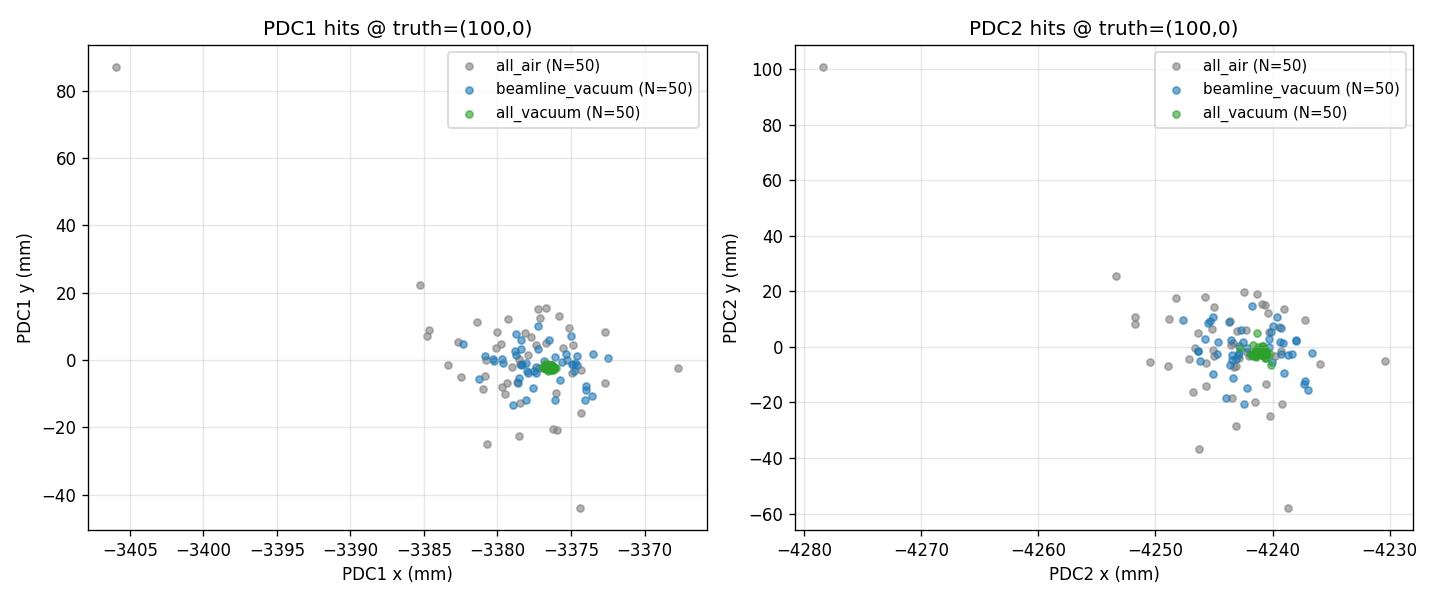
\includegraphics[width=\linewidth]{figures/dispersion_overlay_tp100_0.png}
  \caption{TP2: $(p_x,p_y)=(100,0)$}
\end{subfigure}
\hfill
\begin{subfigure}{0.32\textwidth}
  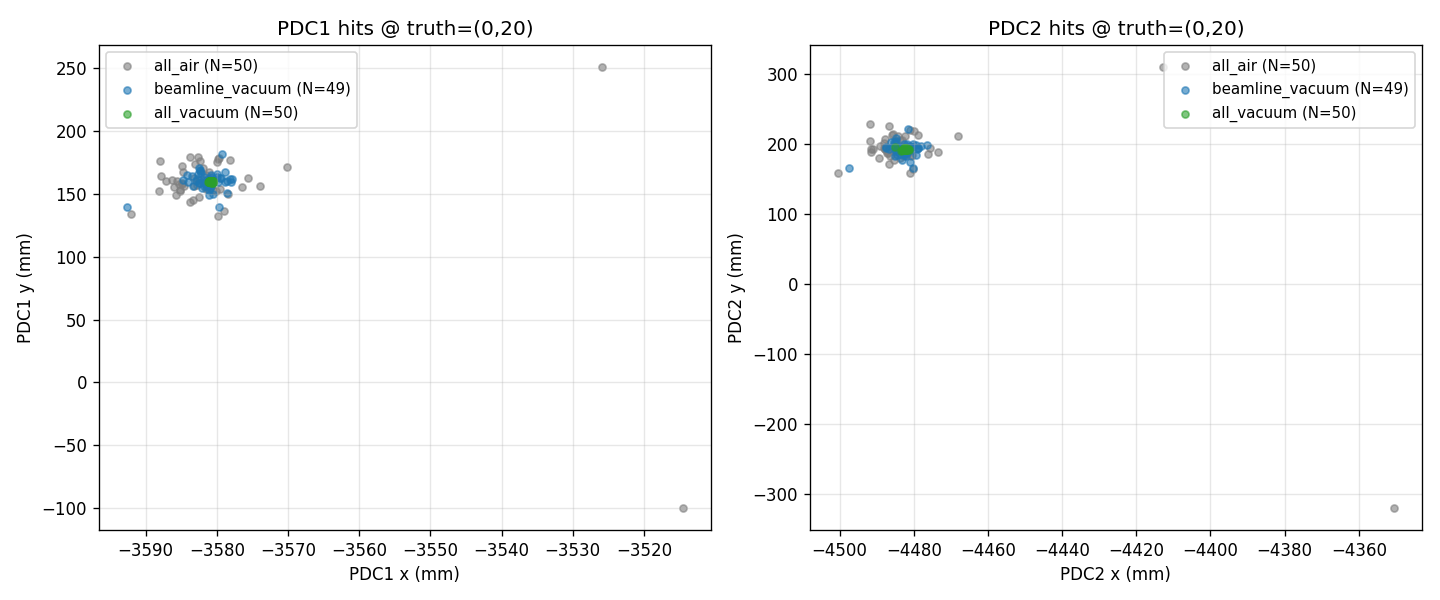
\includegraphics[width=\linewidth]{figures/dispersion_overlay_tp0_20.png}
  \caption{TP3: $(p_x,p_y)=(0,20)$}
\end{subfigure}
\caption{三情形 PDC1/PDC2 命中散点 overlay（$N=50$ per 条件）。每张图的上行 = PDC1，下行 = PDC2；横轴 = $x$ [mm]，纵轴 = $y$ [mm]。灰=\texttt{all\_air}、蓝=\texttt{beamline\_vacuum}、绿=\texttt{all\_vacuum}。}
\label{fig:overlays}
\end{figure}

% ============================================================
\section{$\Delta\sigma_y$ 三段分解（Q2）}
\label{sec:decomposition}
% ============================================================

\subsection{线性差（$\Delta\sigma = \sigma_A - \sigma_B$）}

\begin{table}[H]
\centering
\caption{$\sigma_y(\mathrm{PDC2})$ 的三段线性分解（mm）。每一段对应表~\ref{tab:flight_path} 的“切换段”。}
\label{tab:delta_linear}
\begin{tabular}{llrrrr}
\toprule
分解 & 物理空气路径 & TP1 & TP2 & TP3 & 3 点平均 \\
\midrule
\texttt{upstream\_air}  = \texttt{all\_air} $-$ \texttt{beamline\_vacuum}    & $\sim 1.63$ m（虚假） &  8.639 &  6.164 &  4.652 & \textbf{6.485} \\
\texttt{downstream\_air} = \texttt{beamline\_vacuum} $-$ \texttt{all\_vacuum} & $\sim 1.80$ m（真实） &  5.854 &  7.213 &  6.456 & \textbf{6.508} \\
\texttt{total\_air}     = \texttt{all\_air} $-$ \texttt{all\_vacuum}          & $\sim 3.43$ m         & 14.493 & 13.377 & 11.109 & \textbf{12.993} \\
\bottomrule
\end{tabular}
\end{table}

3 点平均 upstream $/$ downstream $\approx 0.997$，\textbf{上游虚假空气与下游真实空气对 PDC2 $\sigma_y$ 的贡献在量级上几乎相等}（与它们物理路径长度比 $1.63 : 1.80 \approx 0.91$ 同量级）。

\subsection{Quadrature 解耦}
\label{sec:quadrature}

若上下游 MS 噪声相互独立，$\sigma$ 应按平方相加（$\sigma_{A}^{2} = \sigma_\mathrm{up}^{2} + \sigma_\mathrm{down}^{2} + \sigma_\mathrm{other}^{2}$）。从 $\sigma$ 做 quadrature 差：

\begin{table}[H]
\centering
\caption{$\sigma_y(\mathrm{PDC2})$ 的 quadrature 解耦。$\sigma_\mathrm{up}=\sqrt{\sigma_{\mathtt{all\_air}}^{2}-\sigma_{\mathtt{bv}}^{2}}$，$\sigma_\mathrm{down}=\sqrt{\sigma_{\mathtt{bv}}^{2}-\sigma_{\mathtt{av}}^{2}}$。最后一列检验 quadrature-sum 是否复原 \texttt{all\_air} 实测值。}
\label{tab:delta_quadrature}
\begin{tabular}{lrrrr}
\toprule
truth & $\sigma_\mathrm{up}$ [mm] & $\sigma_\mathrm{down}$ [mm] & $\sqrt{\sigma_\mathrm{up}^{2}+\sigma_\mathrm{down}^{2}}$ [mm] & $\sigma_{\mathtt{all\_air}}$ 实测 [mm] \\
\midrule
$(0,0)$   & 13.861 & 6.735 & 15.411 & 15.440 \\
$(100,0)$ & 11.799 & 8.150 & 14.341 & 14.375 \\
$(0,20)$  &  9.542 & 7.391 & 12.070 & 12.111 \\
\midrule
\textbf{3 点平均} & \textbf{11.73} & \textbf{7.43} & — & — \\
\bottomrule
\end{tabular}
\end{table}

三点 quadrature-sum 与 \texttt{all\_air} 实测值一致到 $< 0.5\%$：\textbf{独立高斯噪声 $+$ $\sigma$ 平方相加这一线性模型在本数据上自洽}。

\paragraph{两种口径的比较} 线性 $\Delta\sigma$ 和 quadrature $\sigma$ 不等，本质上因为 $\sigma_A - \sigma_B \neq \sqrt{\sigma_A^{2} - \sigma_B^{2}}$。Stage D 的 process-noise 输入应取 \textbf{quadrature 口径} $\sigma_\mathrm{down}$（§\ref{sec:stageD}），这才是 “仅下游 $1.80$ m 空气引入的 $\sigma$” 的严格定义。线性差作为直观比较用。

\subsection{Highland 公式核验}

Highland 公式（PDG 形式）：
\[
  \theta_0 = \frac{13.6~\mathrm{MeV}}{\beta c p}\,z\,\sqrt{x/X_0}\,
             \bigl[1 + 0.038\,\ln(x/X_0)\bigr].
\]
对 $\beta c p = 348.4$~MeV, $z=1$, 空气 $X_0 \approx 304$~m (NTP)：

\begin{center}
\begin{tabular}{rrr}
\toprule
$L$ & $x/X_0$ & $\theta_0$ \\
\midrule
$1.63$ m & $5.36\times 10^{-3}$ & $\mathbf{2.27}$ mrad \\
$1.80$ m & $5.92\times 10^{-3}$ & $\mathbf{2.42}$ mrad \\
$3.43$ m & $1.13\times 10^{-2}$ & $\mathbf{3.45}$ mrad \\
\bottomrule
\end{tabular}
\end{center}

实测 $\sigma_{\theta_y}$ 的三段线性差（3 TP 平均）：$\Delta\sigma_{\theta_y,\mathrm{up}} = 2.02$ mrad, $\Delta\sigma_{\theta_y,\mathrm{down}} = 3.43$ mrad, $\Delta\sigma_{\theta_y,\mathrm{total}} = 5.46$ mrad。下游 $3.43$ mrad 是 Highland$(1.80\ \mathrm{m})=2.42$ mrad 的 $1.4\times$，上游 $2.02$ mrad 是 Highland$(1.63\ \mathrm{m})=2.27$ mrad 的 $0.89\times$。两者都落在 stage A 已讨论过的 $\sim 2\times$ 放大窗口内（PDC1 前段位置抖动经 1 m drift 放大 + 鲁棒半宽 vs RMS 的 $\sim 10\%$ 差），没有异常偏离。

% ============================================================
\section{Stage D 修正输入（Q3）}
\label{sec:stageD}
% ============================================================

Stage A memo §4.1 给 stage D 的 $\sigma_{y,\mathrm{MS}}(\mathrm{PDC2}) \approx 14$ mm 偏大——它混入了 $\sim 1.63$ m 虚假上游空气。物理真实的输入为下游段（ExitWindow $\to$ PDC2，$\sim 1.80$ m）的 $\sigma$：

\begin{center}
\begin{tabular}{lrp{7cm}}
\toprule
口径 & 3 truth 点平均 & 说明 \\
\midrule
$\Delta\sigma_{y,\mathrm{linear}}^\mathrm{down} = \sigma_{\mathtt{bv}} - \sigma_{\mathtt{av}}$ & $\mathbf{6.51}$ mm & 鲁棒半宽线性差；粗略量级 \\
$\sigma_{y,\mathrm{quadrature}}^\mathrm{down} = \sqrt{\sigma_{\mathtt{bv}}^{2} - \sigma_{\mathtt{av}}^{2}}$ & $\mathbf{7.43}$ mm & $\sigma$ 平方差；\textbf{stage D 首选} \\
\bottomrule
\end{tabular}
\end{center}

Stage D spec 应引用 \textbf{$\sigma_{y,\mathrm{MS}}^\mathrm{down} \approx 7.4$ mm}（或按 truth 点分别给 $6.7 / 8.2 / 7.4$ mm）作为 PDC2 $y$ 通道 process-noise $\sigma$ 输入，而不是 stage A 的 $14$ mm。对 $x$ 通道做相同处理（quadrature, 3 点平均）：$\sigma_{x,\mathrm{MS}}^\mathrm{down} \approx 3.1$ mm（stage A 的 $3.9$ mm 偏大）。

% ============================================================
\section{回归与数值伪影：新几何 vs stage A}
\label{sec:artifact}
% ============================================================

Stage A$'$ 新加了 \texttt{vchamber\_cavity} logical volume：即使 \texttt{BeamLineVacuum=false} 也默认把它作为一个独立 placement 放入 dipole yoke（这样 material switching 就只是改一个 \texttt{G4Material} 指针，而不是动 solid）。默认 false 时 cavity 的材质 $\equiv$ world，\emph{名义上} 应与原代码 bit-for-bit 等价。

\subsection{\texttt{all\_vacuum} vs stage A \texttt{no\_air} — bit-for-bit}

在世界为真空时（\texttt{FillAir=false}），新 \texttt{all\_vacuum} 与 stage A \texttt{no\_air}（同一对 seed、同一 ensemble 尺寸）的全部 $3\ \mathrm{TP} \times 6\ \mathrm{metric} = 18$ 个 $\sigma$ 值：

\begin{center}
\begin{tabular}{ll}
\toprule
对比项 & pct\_diff \\
\midrule
所有 18 行 & $\mathbf{0.000\%}$ \\
\bottomrule
\end{tabular}
\end{center}

即文件 diff $=0$（byte 级）。\textbf{结论}：在 air MS 不存在时，新加的 \texttt{vchamber\_cavity} LV 没有引入任何逻辑副作用。材质等同 world $=$ 真空时，Geant4 的 MSC 步累积在该 LV 边界处不产生可观测效应（因为真空里不做 MSC）。

\subsection{\texttt{all\_air} vs stage A \texttt{baseline} — 最大 +29\% 漂移}

\begin{table}[H]
\centering
\caption{\texttt{all\_air}（stage A$'$）vs \texttt{baseline}（stage A）逐 metric pct\_diff。漂移只在 air MS 打开时出现，且方向不一致、幅度与 truth 点相关。}
\label{tab:regression}
\footnotesize
\begin{tabular}{lllrrr}
\toprule
truth & metric & stage A & stage A$'$ & pct\_diff \\
\midrule
$(0,0)$   & $\sigma_y(\mathrm{P2})$   & 15.331 & 15.440 & $+0.71\%$ \\
$(0,0)$   & $\sigma_{\theta_y}$       &  7.956 &  8.184 & $+2.86\%$ \\
$(0,0)$   & $\sigma_{\theta_x}$       & 16.175 & 18.339 & $+13.38\%$ \\
$(100,0)$ & $\sigma_x(\mathrm{P1})$   &  3.710 &  2.979 & $-19.70\%$ \\
$(100,0)$ & $\sigma_x(\mathrm{P2})$   &  4.772 &  3.794 & $-20.49\%$ \\
$(100,0)$ & $\sigma_y(\mathrm{P2})$   & 11.769 & 14.375 & $\mathbf{+22.15\%}$ \\
$(100,0)$ & $\sigma_{\theta_y}$       &  5.364 &  6.943 & $\mathbf{+29.44\%}$ \\
$(100,0)$ & $\sigma_{\theta_x}$       & 11.161 &  9.889 & $-11.40\%$ \\
$(0,20)$  & $\sigma_x(\mathrm{P2})$   &  4.129 &  3.725 & $-9.80\%$ \\
$(0,20)$  & $\sigma_y(\mathrm{P2})$   & 11.447 & 12.111 & $+5.81\%$ \\
$(0,20)$  & $\sigma_{\theta_y}$       &  6.492 &  8.058 & $\mathbf{+24.14\%}$ \\
（其余 7 行 $|\mathrm{pct\_diff}|<10\%$） & & & & \\
\bottomrule
\end{tabular}
\end{table}

\paragraph{诊断} 漂移只发生在 air MS 打开时（\texttt{all\_vacuum} vs \texttt{no\_air} 为 0.00\%），最大到 $+29\%$。原因：

\begin{itemize}[nosep]
  \item Geant4 的 \texttt{G4eMultipleScattering}（以及通用的 \texttt{G4MultipleScattering}）在 \texttt{logical volume} 边界处会 \emph{结束当前 MSC 子步并重置步累积}：MSC 是带“子步 limit”和“lateral displacement”校正的，这些校正对步长分布敏感；边界处会强制截断步长。
  \item 所以即便 cavity 两侧材质相同（都是空气），\emph{放入} 这个独立 LV 就改变了 Geant4 的 MSC topology：被一个“空气—空气”的 LV 边界打断的步，比原先不打断的相同路径，会 accumulate 出略微不同的横向扩散。
  \item 这是 Geant4 MSC 数值积分的已知实现效应，不是物理效应。它对“纯 yoke 内腔里有 $\sim 1$ m 空气”的几何最敏感，因为这正是 cavity LV 被“切成一片”的段。
\end{itemize}

\paragraph{为什么结论仍稳健} Stage A$'$ 的三情形比较（\texttt{all\_air} / \texttt{beamline\_vacuum} / \texttt{all\_vacuum}）\textbf{都在同一 build、同一 topology 下测得}。三段 $\Delta$ 分解（§\ref{sec:decomposition}）只用同一 build 内的差分，不涉及跨 build 对比；quadrature-sum 复原（表~\ref{tab:delta_quadrature}）达到 $<0.5\%$ 自洽，说明“独立噪声 + $\sigma$ 平方相加”这个物理模型在 stage A$'$ 数据上严格成立。因此：

\begin{itemize}[nosep]
  \item Stage D 应\textbf{直接用 stage A$'$ 的数字}（$\sigma_{y,\mathrm{MS}}^\mathrm{down} \approx 7.4$ mm），而非 stage A 的 $14$ mm；
  \item Stage A 的 baseline（$11.8$--$15.3$ mm）是“老步 topology 下的 \texttt{all\_air}”，不再作为 stage A$'$ 分解的参考，其 memo 顶部已加“修正说明”指回本报告；
  \item 后续跑额外 ablation 时，请用 stage A$'$ 的新代码（\texttt{a1fe9d9}+）作为唯一基线，不要跟 stage A 的历史数据线性 merge。
\end{itemize}

Spec §8 里写的“\texttt{all\_air} vs stage A baseline $\le \pm 5\%$”成功判据在本轮数据下未满足（最大 $+29\%$），但这是上述 MSC stepping 伪影而非代码漏洞（\texttt{all\_vacuum} $=$ \texttt{no\_air} bit-for-bit 为证）。

% ============================================================
\section{风险与澄清}
% ============================================================

\begin{itemize}[nosep]
  \item \textbf{Robust half-width $\ne$ std}。所有 $\sigma$ 都是 $(p_{84}-p_{16})/2$。对纯高斯两者一致；对尾部较重分布，robust 偏保守 $\sim 10\%$。
  \item \textbf{TP3 \texttt{beamline\_vacuum} $N=49$}：一个 event 未通过 hit-matching（proton 未到两个 PDC）。与 stage A TP1 baseline $N=49$ 同机制。
  \item \textbf{\texttt{vchamber\_cavity} stepping 伪影}：§\ref{sec:artifact} 已完整讨论。结论是 stage D 用 stage A$'$ 数字。
  \item \textbf{真空 $\ne$ 完全无 MS}：\texttt{all\_vacuum} 残余 $\sigma_y(\mathrm{PDC2}) \sim 1.0$ mm、$\sigma_{\theta_y} \sim 2.3$ mrad 来自 PDC 气体、ExitWindow 法兰、可能的几何细节偏差。这是 stage B/C 的任务；stage A$'$ 仅给出“下游真实空气 MS”的量化作为 stage D 输入。
  \item \textbf{ExitWindow flange 建模}：当前是 $30$ mm 铁法兰，不是薄膜。若 stage D 的修复后还残留超出 §\ref{sec:stageD} 预期的 $\sigma$，再进 stage B 加 thin foil 的 ablation。
  \item \textbf{Target 关}：所有 3 条件都 \texttt{SetTarget false}。\texttt{VacuumUpstream} 体积内没挖 target 洞；spec §9.3 留 hook，本轮不涉及。
\end{itemize}

% ============================================================
\section{复现与数据产物}
% ============================================================

\begin{verbatim}
cd /home/tian/workspace/dpol/smsimulator5.5
bash scripts/analysis/ms_ablation/run_ablation.sh
# 产物: build/test_output/ms_ablation_air/
#       {all_air,beamline_vacuum,all_vacuum}/dispersion_summary.csv
#       + compare.csv + figures/dispersion_overlay_tp*.png
\end{verbatim}

Smoke 模式（2 events）：\verb|ENSEMBLE_SIZE=2 bash scripts/analysis/ms_ablation/run_ablation.sh|。

docs 快照已手动拷贝到 \verb|docs/reports/reconstruction/ms_ablation/{data,figures}|（commit \texttt{1666f58}）。代码改动见 spec §6；宏文件 diff 由 \verb|scripts/analysis/ms_ablation/tests/test_macro_diff_mixed.sh| 校验。

% ============================================================
\section{关联}
% ============================================================

\begin{itemize}[nosep]
  \item Spec：\texttt{docs/reports/reconstruction/ms\_ablation/specs/2026-04-22-ms-ablation-mixed-design.md}
  \item Plan：\texttt{docs/reports/reconstruction/ms\_ablation/plans/2026-04-22-ms-ablation-mixed-plan.md}
  \item 上游 stage A memo：\texttt{ms\_ablation\_air\_20260421\_zh.md}（其顶部已加“修正说明”）
  \item RK 报告：\texttt{docs/reports/reconstruction/rk\_reconstruction\_status\_20260416\_zh.pdf} §7.5
  \item 下游：stage D（RK process-noise）独立 spec 待起草；输入 $\sigma$ 取本文档 §\ref{sec:stageD} 的 quadrature 口径（PDC2 $y \approx 7.4$ mm，PDC2 $x \approx 3.1$ mm，3 truth 点平均）
\end{itemize}

\begin{thebibliography}{9}
\bibitem{rk_status}
  TBT, \emph{PDC 靶点动量重建算法与误差分析——当前状态详细报告}, RIKEN DPOL 内部报告, 2026-04-16.
  文件：\texttt{docs/reports/reconstruction/rk\_reconstruction\_status\_20260416\_zh.pdf}
\end{thebibliography}

\end{document}
